\documentclass[tikz,border=4pt]{standalone}
\usepackage[T1]{fontenc}
\usepackage{lmodern}
\usepackage{amsmath}
% Shared TikZ style for the report figures.
% Colours follow the Okabe-Ito palette, which stays distinguishable under the
% common forms of colour-vision deficiency. Every colour-coded element also
% carries a text label, so no figure depends on colour alone.
\usetikzlibrary{arrows.meta,positioning,fit,calc,backgrounds,decorations.pathreplacing,shapes.geometric}

\definecolor{oiOrange}{HTML}{E69F00}
\definecolor{oiSky}{HTML}{56B4E9}
\definecolor{oiGreen}{HTML}{009E73}
\definecolor{oiYellow}{HTML}{F0E442}
\definecolor{oiBlue}{HTML}{0072B2}
\definecolor{oiVerm}{HTML}{D55E00}
\definecolor{oiPurple}{HTML}{CC79A7}
\definecolor{oiGray}{HTML}{6E6E6E}

\colorlet{corTreino}{oiBlue!22}
\colorlet{corValid}{oiGreen!30}
\colorlet{corTeste}{oiOrange!45}
\colorlet{corControle}{oiPurple!35}

\tikzset{
  >=Stealth,
  bloco/.style={draw=black!70, rounded corners=1.5pt, minimum height=0.62cm,
    inner sep=2pt, font=\sffamily\fsz, align=center},
  treino/.style={bloco, fill=corTreino},
  valid/.style={bloco, fill=corValid},
  teste/.style={bloco, fill=corTeste, thick},
  etapa/.style={draw=black!70, rounded corners=3pt, fill=black!4,
    text width=4.3cm, align=center, inner sep=4pt, font=\sffamily\fsz},
  nota/.style={font=\sffamily\fsz, align=left, text=black!80},
  titulo/.style={font=\sffamily\fst\bfseries, anchor=west},
  seta/.style={->, thick, black!70},
  regiao/.style={draw=black!50, dashed, rounded corners=4pt},
}

% Absolute font sizes, so a figure looks the same standalone (10 pt class) and
% inside the 11 pt report.
\providecommand{\fsx}{\fontsize{5.5}{6.5}\selectfont}
\providecommand{\fsz}{\fontsize{7}{8.5}\selectfont}
\providecommand{\fst}{\fontsize{9}{11}\selectfont}

\begin{document}
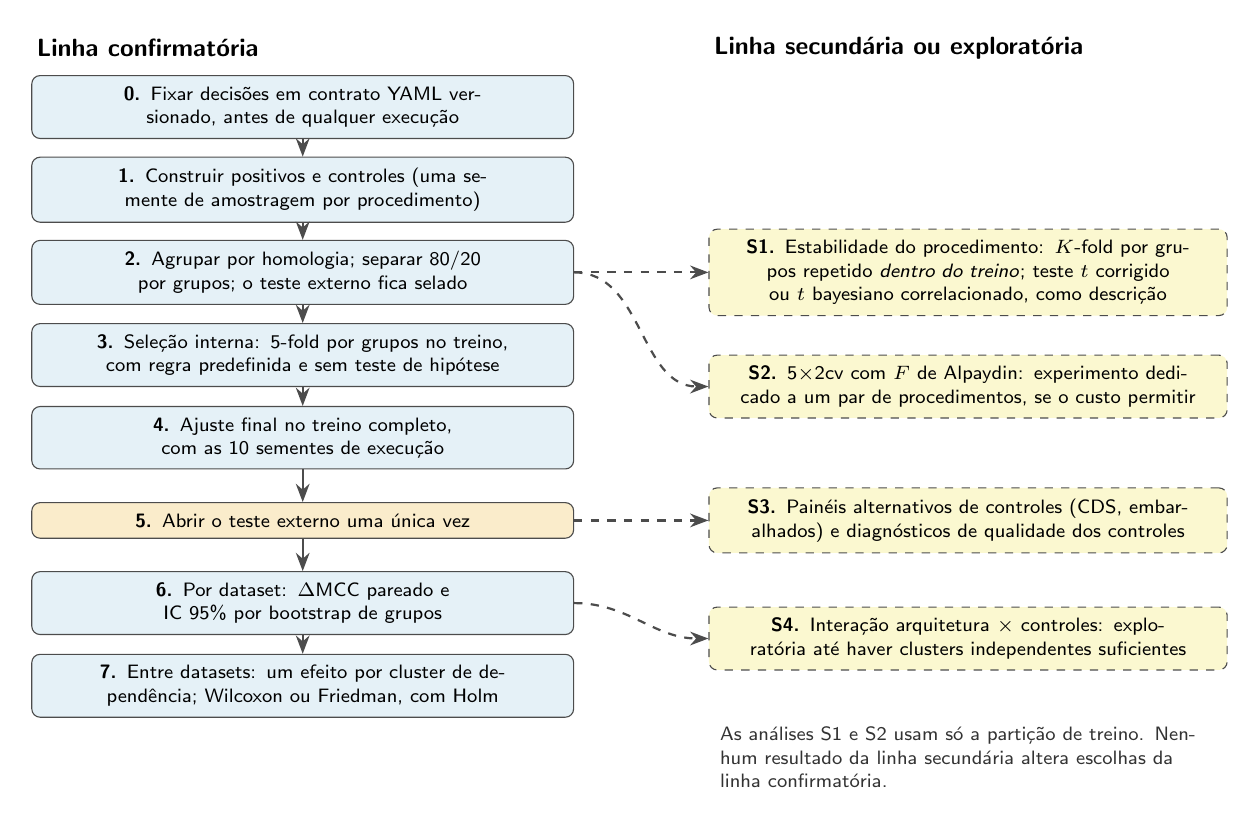
\begin{tikzpicture}[
  conf/.style={etapa, text width=6.6cm, fill=oiBlue!10},
  expl/.style={etapa, text width=6.3cm, fill=oiYellow!25, dashed},
  ]
  \node[titulo] at (0,0.75) {Linha confirmatória};
  \node[titulo] at (8.6,0.75) {Linha secundária ou exploratória};
  \node[conf] (c0) at (3.5,0)     {\textbf{0.} Fixar decisões em contrato YAML versionado, antes de qualquer execução};
  \node[conf] (c1) at (3.5,-1.05) {\textbf{1.} Construir positivos e controles (uma semente de amostragem por procedimento)};
  \node[conf] (c2) at (3.5,-2.1)  {\textbf{2.} Agrupar por homologia; separar 80/20 por grupos; o teste externo fica selado};
  \node[conf] (c3) at (3.5,-3.15) {\textbf{3.} Seleção interna: 5-fold por grupos no treino, com regra predefinida e sem teste de hipótese};
  \node[conf] (c4) at (3.5,-4.2)  {\textbf{4.} Ajuste final no treino completo, com as 10 sementes de execução};
  \node[conf, fill=corTeste!45] (c5) at (3.5,-5.25) {\textbf{5.} Abrir o teste externo uma única vez};
  \node[conf] (c6) at (3.5,-6.3)  {\textbf{6.} Por dataset: $\Delta$MCC pareado e IC 95\% por bootstrap de grupos};
  \node[conf] (c7) at (3.5,-7.35) {\textbf{7.} Entre datasets: um efeito por cluster de dependência; Wilcoxon ou Friedman, com Holm};
  \foreach \a/\b in {c0/c1,c1/c2,c2/c3,c3/c4,c4/c5,c5/c6,c6/c7} { \draw[seta] (\a) -- (\b); }

  \node[expl] (e1) at (11.95,-2.1) {\textbf{S1.} Estabilidade do procedimento: $K$-fold por grupos repetido \emph{dentro do treino}; teste $t$ corrigido ou $t$ bayesiano correlacionado, como descrição};
  \node[expl] (e2) at (11.95,-3.55) {\textbf{S2.} 5$\times$2cv com $F$ de Alpaydin: experimento dedicado a um par de procedimentos, se o custo permitir};
  \node[expl] (e3) at (11.95,-5.25) {\textbf{S3.} Painéis alternativos de controles (CDS, embaralhados) e diagnósticos de qualidade dos controles};
  \node[expl] (e4) at (11.95,-6.75) {\textbf{S4.} Interação arquitetura $\times$ controles: exploratória até haver clusters independentes suficientes};
  \draw[seta, dashed] (c2.east) -- (e1.west);
  \draw[seta, dashed] (c2.east) to[out=0,in=180] (e2.west);
  \draw[seta, dashed] (c5.east) -- (e3.west);
  \draw[seta, dashed] (c6.east) to[out=0,in=180] (e4.west);
  \node[nota, text width=6.3cm, anchor=north] at (11.95,-7.75)
    {As análises S1 e S2 usam só a partição de treino. Nenhum resultado da linha secundária altera escolhas da linha confirmatória.};
\end{tikzpicture}
\end{document}
